\chapter{仿真实验场景的设计与构建}

仿真平台选择与仿真环境的搭建在交通研究中扮演着非常重要的角色。随着城市化进程的不断加速和交通需求的不断增长,城市交通系统的规划和管理变得越来越复杂和困难。传统的基于观察和统计数据的研究方法已经无法满足交通系统优化和决策的需求,因此交通仿真技术应运而生。

交通仿真是通过计算机技术对交通系统进行建模、仿真和分析,以获得交通系统行为和性能方面的信息。通过仿真平台的选择和搭建,可以对不同的交通系统进行模拟和测试,以评估不同交通系统的性能和效果。仿真平台可以帮助交通研究者理解交通系统的复杂性和动态性,预测未来交通系统的发展趋势,并提出优化方案和决策建议。

在交通研究中,不同的仿真平台有着各自的优缺点和适用范围。例如,商业软件VISSIM可以模拟更加复杂和精细的交通系统,但是需要购买授权和付费,对于一些小型和非营利性项目来说,成本较高。相比之下,SUMO是一款开源的、免费的仿真平台,可以轻松地进行定制和扩展,因此被广泛应用于学术界和非营利组织中。

在仿真平台的搭建方面,需要根据具体的研究问题和场景进行选择和设计。例如,在仿真场景的选择方面,需要考虑到不同的交通模式、路段的特点和流量情况等因素。在路网的编辑和生成方面,需要考虑到交通规划和设计的要求,并对道路的连接、交叉口的设计等进行合理的规划和调整。在流量的生成方面,需要根据实际情况进行仿真和预测,以准确地反映交通系统的行为和性能。

第三章将主要介绍仿真实验场景的设计与构建,首先分析不同仿真平台的优缺点,以及在深度强化学习的出行模式和时间选择研究中为何选择SUMO作为仿真平台。接着,详细介绍基于SUMO仿真平台的城市交通仿真平台,包括平台设计目标、功能模块简介。最后,完成本文实验所需场景的选择与搭建、路网的编辑与生成、出行模式的设计和流量的生成等方面。

\section{城市交通仿真平台的可行性分析}

\subsection{Vissim介绍}

VISSIM是由德国PTV(Planung Transport Verkehr AG)公司开发的一款功能强大的交通模拟软件,广泛应用于交通规划、设计、管理等领域。其模拟能力可以涵盖各种复杂的交通场景,如城市道路、高速公路、交叉口、公共交通、交通流、交通信号控制、公共交通路线规划和车辆路径规划等。

VISSIM的建模功能非常强大,用户可以使用图形用户界面轻松创建交通场景,包括道路、交叉口和公共交通路线等。用户还可以调整交通流率、车辆类型、行人流量和其他参数,以建立一个真实的交通网络。智能交通生成器使用真实的交通数据,为一天中的不同时段、工作日和周末创建真实的交通流模式。同时,用户还可以根据自己的需要进行定制,调整交通量、速度和其他参数,以快速创建虚拟的交通场景。

VISSIM的仿真模拟功能是其最核心的功能之一,用户可以通过VISSIM的仿真引擎高度准确地模拟各种交通场景,从简单的交叉口到复杂的城市网络。仿真引擎可以生成实时交通数据,如车辆速度、行驶时间和延迟时间等。用户可以对交通管理策略进行模拟,如交通信号控制、公共交通路线规划和车辆路径规划,并评估不同交通管理策略的性能,比较不同方案的效果,做出明智的决策。同时,用户可以通过虚拟实验,得出真实世界中的交通流动规律,从而更好地解决实际问题。

VISSIM还提供了强大的分析功能,用户可以分析和可视化模拟结果,生成大量的图表和表格来分析交通流量、拥堵情况、车辆行驶时间、车辆速度和其他指标。分析功能还允许用户比较不同交通管理策略的性能,评估不同参数对交通流的影响。通过VISSIM的分析功能,用户可以更全面、更深入地了解交通流动规律,并进一步优化交通系统的设计和管理。

整体来说,VISSIM是一款功能强大的交通模拟软件,可以广泛应用于交通规划、设计、管理等领域。VISSIM的建模、仿真和分析功能都非常强大,可以帮助用户高度准确地模拟各种交通场景,评估交通管理策略的性能,并优化交通系统的设计和管理。作为交通专业人员、研究人员和政策制定者的重要工具,VISSIM为实现更安全、更高效和可持续的未来交通系统做出了巨大的贡献。


\subsection{SUMO介绍}

SUMO(Simulation of Urban Mobility)是一款由德国科研机构DLR开发的开源交通仿真软件,广泛应用于城市交通规划、交通管理、交通研究等领域。该软件旨在提供高效、可扩展和高度自定义的交通仿真,以及良好的可视化和数据输出。SUMO具有开放性、高可靠性、高可扩展性和良好的可视化效果等特点,成为交通仿真领域的重要工具之一。

SUMO的基本功能包括建模、仿真技术和可视化。用户可以使用该软件创建虚拟交通网络,并定义网络中的道路布局、交通流和车辆类型。SUMO使用微观交通模拟引擎,可以模拟各种交通场景,如车辆路线、公共交通和行人运动,并生成实时交通数据。用户可以通过SUMO的图形用户界面对模拟结果进行可视化,也可以生成各种图表和表格总结模拟结果。

除了基本功能外,SUMO还提供定制功能、多模式仿真、优化功能、并行化和集成等高级功能。用户可以通过SUMO定义影响模拟的不同参数、自定义脚本、创建自定义的车辆模型,并将其导入到模拟中。该软件支持多模式模拟,如汽车、公交车、火车和自行车,用户可以评估不同交通方式的性能,并对不同的交通计划进行比较。SUMO还提供优化功能,可以优化交通信号灯时间、车辆路线和公共交通时间表,找到最佳的交通管理策略和交通计划。SUMO提供并行化功能,允许用户在多个处理器上运行模拟,加快模拟时间,并模拟更大的交通网络。此外,SUMO可以与其他软件工具集成,如交通流模型、地理信息系统(GIS)和数据分析工具,为用户提供一套全面的工具来模拟和分析各种交通情况。

总之,SUMO是一个功能强大、用途广泛的模拟软件,为用户提供了一套全面的工具来模拟和分析各种交通情况。该软件支持多模式交通的模拟,包括汽车、公交车、自行车和行人,它还提供了一些高级功能,如交通需求生成、交通信号控制和车辆路由。SUMO的灵活架构和开源代码库使其成为研究人员、交通专业人士和需要高度可定制模拟工具的决策者的热门选择。SUMO有能力生成真实的交通数据,并提供对交通系统性能的洞察力,在设计、优化和评估交通系统方面发挥了关键作用,以实现更安全、更高效和可持续的未来。

\subsection{MATSim介绍}

MATSim是一款由瑞士苏黎世联邦理工学院(ETH Zurich)开发的开源交通仿真软件。该软件基于代理人建模,能够模拟不同交通方式的选择和相互作用,以及不同交通场景下的个人行为和整个交通系统的运行情况。此外,MATSim提供了全面的可视化工具,使用户可以实时查看模拟的结果,包括交通流量、旅行时间等重要指标。

MATSim的模块化架构使用户能够根据自己的需求定制软件,以模拟新的运输系统或包括新的功能。这使该软件能够适应不同交通场景的具体要求,并成为研究人员和交通专业人士的热门选择。MATSim还具有开源代码库的特点,允许用户修改软件并将其分发给其他人,使研究人员和交通专业人士能够合作和分享他们的工作。

MATSim是一个功能强大的交通仿真软件,能够模拟多种交通方式和不同的交通场景,使用户能够评估不同交通系统的性能,并优化城市或区域内不同交通方式的使用。该软件已被广泛测试和验证,用于对全球不同城市和地区的交通系统进行建模和模拟,证明了其对交通系统进行精确建模和模拟的能力。MATSim在设计、优化和评估交通系统以实现更安全、更高效和可持续的未来方面发挥了关键作用。

总之,MATSim是一款功能强大、用途广泛的交通仿真软件,为用户提供了一套全面的工具来模拟和仿真不同的交通场景。该软件的模块化架构、多模式模拟能力、先进的可视化功能和开源代码库使其成为研究人员和交通专业人士的热门选择。MATSim能够准确地模拟交通系统并评估不同交通方案的性能,在设计、优化和评估交通系统以实现更安全、更高效和可持续的未来方面发挥了关键作用。


\subsection{仿真平台的选择}

通过对三种主流交通仿真平台的介绍,表\ref{tab:3_1}总结梳理了各个仿真平台的优缺点。

\renewcommand{\arraystretch}{1.5} % 使表格行间距加大1.5倍
\begin{table}[htbp]
\centering
\caption{不同仿真软件的对比}
\label{tab:3_1}
\begin{tabular}{cll}
\toprule
仿真软件 & \multicolumn{1}{c}{优点}       & \multicolumn{1}{c}{缺点}     \\
\midrule
VISSIM                       & \parbox[t]{5.5cm}{城市和区域交通系统、交通行为建模、支持多种交通模式、交通流量和排放量测量评估}      & \parbox[t]{5.5cm}{商业软件、非机动车和行人交通模式处理能力有限、复杂交通场景模拟效果可能不够准确、缺乏开源模型和工具 }                       \\
SUMO                      & \parbox[t]{5.5cm}{速度快、处理大规模交通网络、开放性、开源模型和工具、多种交通模式和路段可调整性}    & \parbox[t]{5.5cm}{交通行为建模较为简单、非机动车和行人交通模式处理能力有限、缺少全面的可视化工具}              \\ 
MATSim                    & \parbox[t]{5.5cm}{模拟多种交通方式和不同的交通场景、模块化架构、提供全面的可视化工具、开源代码库}   & \parbox[t]{5.5cm}{对于大规模交通网络的处理能力有限、个人行为的细节模拟较为复杂、某些交通模式和场景的支持仍不够全面、模拟速度相对较慢}              \\
\bottomrule
\end{tabular}
\end{table}


SUMO、VISSIM和MATSim是三款常用的交通仿真软件,它们各自具有一定的优劣势。其中,SUMO是一款开源软件,用户可以免费使用和修改,而VISSIM则是商业软件,需要购买授权才能使用。MATSim虽然是开源软件,但其复杂度和使用难度相对较高。因此,使用SUMO平台作为仿真工具,能够在节约成本的前提下实现高质量的仿真。

在仿真速度方面,SUMO的速度相对较快,适合处理大规模交通网络。而VISSIM的仿真速度较慢,在处理大规模网络时效果不如SUMO。MATSim在处理大规模网络时也存在一定的限制。因此,在大规模交通仿真方面,使用SUMO平台可以更快速地生成模拟结果,为交通规划和管理提供更快捷的决策支持。

SUMO还提供了可定制的API和开源模型,便于进行二次开发和扩展,而VISSIM和MATSim的API和模型相对较为封闭,用户的自定义程度较低。这一特点使得SUMO平台能够更好地适应不同仿真需求,提高仿真的灵活性和可扩展性。同时,这也使得SUMO平台成为开发新的交通仿真工具和应用的理想平台,为深度强化学习等新兴技术的应用提供了广阔的发展空间。

除此之外,SUMO对非机动车和行人等非机动交通模式的处理能力相对较强,而VISSIM和MATSim在这方面存在一定的局限性。这意味着SUMO平台可以更好地模拟现实交通场景,更准确地预测交通行为和流量,从而为交通规划和管理提供更高效的支持。另外,SUMO平台上已经有相关的研究和开源工具,支持深度强化学习算法的应用。而在VISSIM和MATSim上的应用研究相对较少,缺乏相应的成熟工具和开源库。因此,使用SUMO平台能够方便地借鉴和复用这些成果,提高仿真的效率和准确性。

综上所述,SUMO平台作为一款开源、高效、灵活和可扩展的仿真工具,非常适合用于本文的基于深度强化学习的出行模式和时间选择仿真。


\section{基于SUMO的城市交通仿真平台}

在前一节中,介绍了仿真平台的选择,重点比较了SUMO、VISSIM和MATSim三个交通仿真软件的优缺点,并说明了为何在基于深度强化学习的出行模式和时间选择仿真中,使用SUMO作为仿真平台是一个较为理想的选择。本节将进一步介绍基于SUMO的城市交通仿真平台的设计与构建,其中包含了平台设计目标和功能模块简介两个方面。

\subsection{平台设计目标}


本研究的目的是利用深度强化学习方法研究出行者的出行模式和时间选择行为,并利用出行者的学习行为,实现提高出行效率。为此,我们采用SUMO仿真平台作为我们的仿真工具,以模拟不同的交通环境和交通管理策略。

SUMO仿真平台是一个开源的、高度可定制的交通流量仿真器,支持多种车辆类型和行驶策略,如私家车、公共交通、自行车和行人等。它还提供了一个完整的仿真工具链,包括道路网络编辑器Netedit、仿真器SUMO、交互式仿真器SUMO-GUI和命令行接口TraCI等,支持多种路线选择算法和交通灯控制算法,用户可以根据他们的应用场景选择最适合的算法。然而,如果开发者直接在实验流中调用TraCI而不改进其上的结构以满足实际需求,将会导致代码结构混乱,代码可读性、复用性和扩展性较差等问题,这种方案只适用于简单试验性质的仿真,不能用于系统性的研究工作。因此,SUMO仿真平台的设计目标是为强化学习算法训练和调试不同结构的区域路网提供支持,能够灵活地构造和修改仿真实验的网络道路拓扑结构和环境参数,复现经典深度强化学习算法并提供实验算法流程示例,同时对实时实验和模型数据具有一定的记录和可视化功能。
 

\subsection{功能模块简介}
SUMO包括Netedit、TraCI、SUMO-Tools和SUMO-Plugins四个重要的功能模块。Netedit允许用户创建、编辑和管理道路网络,TraCI允许用户控制车辆和路口的运动和行为。SUMO-Tools用于模拟和评估交通管理策略,SUMO-Plugins用于扩展SUMO的功能和行为。这些功能模块和工具可以相互集成,为用户提供了一个强大和灵活的仿真环境,使得用户可以模拟不同的交通场景和交通管理策略,评估其效果和优化方案,进而提高交通流量的效率和可持续性。

Netedit是SUMO中一个重要的功能模块,用于创建、编辑和管理道路网络。用户可以通过Netedit提供的图形界面添加和编辑道路、路口、车道和交通灯等元素,以模拟不同的交通环境和交通管理策略。同时,Netedit支持多种地图格式,如OpenStreetMap、Google Maps和Bing Maps等。用户可以通过拖放操作和线条绘制工具轻松绘制道路网络。Netedit还提供一些有用的工具,如道路长度和宽度测量工具,帮助用户更准确地绘制道路网络。创建和编辑完成后,用户可以导出Netedit文件以供SUMO-GUI或其他仿真器使用。Netedit还支持Python脚本,用户可以通过编写脚本自动化地创建和编辑道路网络。

TraCI是SUMO中的另一个重要功能模块,它允许用户控制车辆和路口的运动和行为,以模拟不同的交通环境和交通管理策略。TraCI提供了一系列API接口,用户可以通过Python脚本访问和修改仿真器中的车辆和路口状态,如车辆的位置、速度、目标路段和加速度等信息。用户也可以控制车辆的加速、刹车和转向,以及路口的红绿灯和车辆进出等操作。TraCI还支持多种车辆类型和行驶策略,并提供有用的工具和功能,如路网查询、车辆生成和路由规划等,帮助用户更好地控制和管理交通流量。TraCI可以与其他SUMO模块和工具集成,如SUMO-GUI、SUMO-Tools和SUMO-Plugins等,为用户提供更多的定制和扩展能力。

SUMO-Tools是SUMO中用于模拟和评估交通管理策略的功能模块,如交通灯控制和路由优化。SUMO-Tools包括一个流量分析器、一个行驶速度分析器和一个决策支持工具等,用户可以使用它们分析和比较不同的交通管理策略,以评估其效果和优化方案。SUMO-Plugins是SUMO的可扩展模块,允许用户添加自定义的功能和行为,如新的车辆类型、路线选择器、行驶策略和交通管理策略等。SUMO-Plugins可以是Python脚本、C++插件或Java插件等,支持多种路线选择算法和交通灯控制算法。SUMO-Tools和SUMO-Plugins可以与其他SUMO模块和工具集成,如SUMO-GUI和TraCI等,为用户提供更多的定制和扩展能力。使用SUMO-Tools和SUMO-Plugins,用户可以模拟和评估不同的交通管理策略,创建复杂的交通场景,并添加自定义的功能和行为,以满足特定应用程序的需要。SUMO-Tools和SUMO-Plugins为用户提供了一个灵活的仿真环境,使得用户可以针对特定的交通问题和应用场景进行定制和扩展。



\section{实验场景的选择与搭建}

在基于SUMO的城市交通仿真中,实验场景的选择和搭建是十分重要的,它直接决定了仿真结果的可靠性和实用性。实验场景的选择和搭建包括了路网的编辑与生成、出行模式的设计和流量的生成等多个方面。在本节中,将详细介绍如何通过SUMO的功能模块和工具,搭建出逼近真实世界的仿真场景,从而进行有效的交通流量仿真和出行模式探究。

\subsection{路网的编辑与生成}

在本研究中,我们使用SUMO作为交通仿真引擎。SUMO是一个开源的交通仿真软件,支持建模、仿真和分析各种交通场景,包括道路交通、公共交通、自行车交通和行人交通等。

为了研究基于深度强化学习的出行模式和时间选择,我们需要建立一个仿真环境来模拟交通流。这个仿真环境需要选择一个具有典型城市交通结构和各种出行方式的区域进行研究。因此,我们选择了中国苏州市的一个城市区域作为我们的研究对象,该区域面积大约为20平方公里,具有复杂的道路结构和丰富的出行方式,是一个理想的研究对象。图\ref{suzhounet}是仿真场景选取的现实路网区域。

\begin{figure}[htbp]
  \centering
  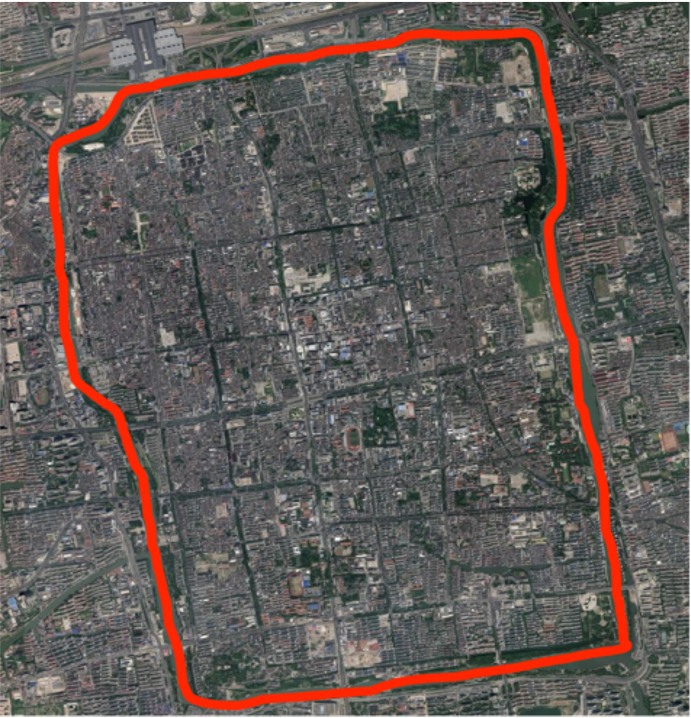
\includegraphics[width=.5\linewidth]{figures/content/suzhounet.png}
  \caption{仿真场景选取区域}
  \label{suzhounet}
\end{figure}

接着通过OpenStreetMap(OSM)来获取苏州市的路网几何和配置信息。OSM是一个开源的地图服务,可以提供全球范围内的地图数据,包括道路、建筑和自然环境等。我们使用OSM提供的数据,利用SUMO软件进行仿真。在建立仿真环境时,我们考虑到苏州市的交通网络的实际情况,并进行了一些修正和调整。添加了一些缺失的路段和交叉口,并对一些道路和交叉口进行了精细调整,以更好地模拟真实的交通流动态。此外,还添加了一些交通规则和限制条件,如车速限制、交通信号灯和路口优先级等,以更真实地模拟交通环境。

最终,我们成功建立了一个具有复杂交通结构和多种出行方式的仿真环境,可以用于研究基于深度强化学习的出行模式和时间选择。通过SUMO的仿真功能,我们可以对不同出行模式和时间选择的影响进行量化分析,帮助我们更好地了解这些问题。图\ref{suzhousumo}是对选取区域使用Netedit模块搭建后的SUMO路网,包含2,423个节点和4,970条路段。

\begin{figure}[htbp]
  \centering
  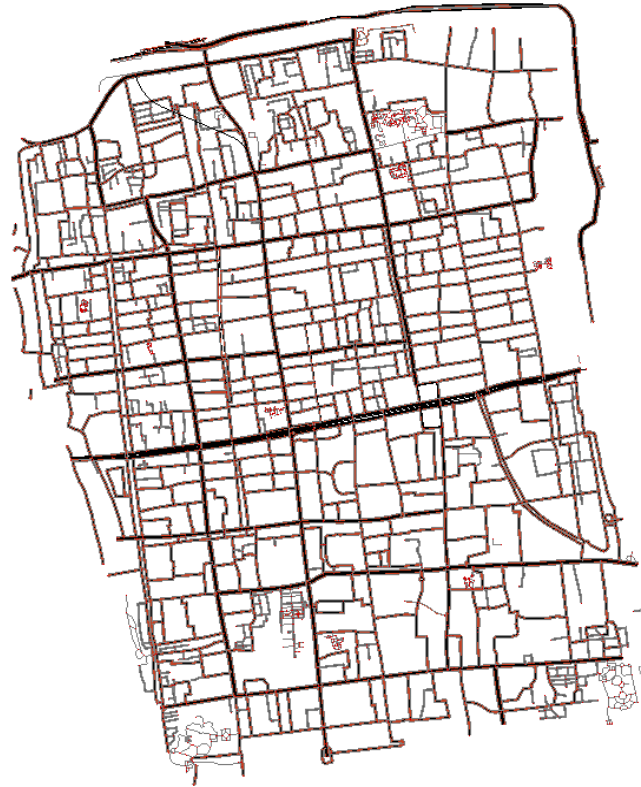
\includegraphics[width=.5\linewidth]{figures/content/suzhousumo.png}
  \caption{SUMO中的仿真路网}
  \label{suzhousumo}
\end{figure}

\subsection{出行模式的设计}

出行模式的设计是交通仿真中的一个重要方面。在本研究中,我们旨在研究深度强化学习在出行模式和出发时间选择方面的应用。因此,我们需要在SUMO交通仿真软件中建立一个具有多种出行方式的仿真环境。

在本研究中,我们考虑了私家车、公共交通(包括公交车和地铁)和自行车三种出行方式。私家车是最常见的出行方式之一,而公共交通和自行车则是城市交通中的重要组成部分。为了实现这种多模式交通网络的仿真,我们需要对这些出行方式进行适当的建模和参数化。

首先,我们需要确定私家车、公共交通和自行车在SUMO仿真中的特征和参数。对于私家车,我们需要考虑其速度、加速度和刹车距离等因素。对于公共交通,我们需要考虑车辆的数量、停靠站点、运营时间和乘客人数等因素。对于自行车,我们需要考虑其速度、加速度和行驶距离等因素。

其次,我们需要将这些特征和参数纳入到SUMO仿真中,以便代理可以在仿真环境中对它们进行操作。对于私家车,我们可以利用SUMO的Car-Following模型来建模其运动行为。对于公共交通,我们可以利用SUMO中的公交车和地铁模型来建模其运营行为。对于自行车,我们可以利用SUMO的Bicycle模型来建模其运动行为。通过将这些模型组合在一起,我们可以实现多种出行方式的仿真。

最后,我们需要在SUMO仿真环境中建立一个多模式交通网络。这个网络需要包括私家车、公共交通和自行车在内的所有出行方式,以便代理可以在仿真环境中对它们进行操作。我们需要将道路、交叉口和停靠站点等元素纳入仿真环境中,并通过SUMO的网络编辑工具对其进行编辑和配置。这样,我们就可以建立一个具有多种出行方式的仿真环境,用于研究基于深度强化学习的出行模式和出发时间选择。

由于我们的仿真区域是一个多模式交通网络,公共交通(包括公交和地铁)也必须被配置。为了实现这一点,我们首先从地图服务应用程序中提取公共交通运营信息,然后进行地图匹配。提取的信息包括线路ID、停靠站或车站ID及其地理位置。这些信息可以通过地图匹配技术与实际地图中的位置进行匹配,从而实现公共交通在仿真环境中的配置。

在本研究中,我们成功地建立了一个具有复杂交通结构和多种出行方式的仿真环境,可以用于研究出行模式和出发时间选择。通过SUMO的仿真功能,我们可以对不同出行模式和出发时间选择的影响进行量化分析,帮助我们更好地了解这些问题。同时,我们还可以通过仿真来测试不同的出行政策和规划方案,以便为决策者提供科学的依据和参考。

为了建立融合公共交通、私家车和自行车的多模式交通网络,我们需要对网络进行适当的编辑和生成。在本研究中,我们使用OpenStreetMap(OSM)来获取网络的几何和配置信息,并将这些信息输入到SUMO中进行仿真。在OSM中,道路、路径、建筑和其他空间要素都被准确地绘制在地图上。SUMO可以将这些信息转换为交通仿真模型,并在模拟中使用它们。同时,我们还需要配置公共交通(包括公交车和地铁)和自行车的路线和停靠点。这些信息可以从地图服务应用程序中提取,并与OSM中的信息进行匹配。

在多模式交通网络中,不同的出行模式需要不同的道路和路径支持。例如,自行车需要有专门的自行车道,而公共交通需要有专门的公交车道和地铁隧道。在网络生成过程中,我们需要将这些要素考虑在内,并将其配置到对应的道路和路径上。这样,在模拟中,不同的出行模式可以根据自己的需求使用不同的道路和路径,从而更好地模拟现实世界中的交通流。

在多模式交通网络中,出行者的出行方式选择涉及到多个变量和因素。例如,私家车出行者可能会考虑到停车地点和停车费用,而公共交通出行者可能会考虑到车站或站点的位置和交通运行时间等。在模型设计中,我们需要考虑到这些因素,以便为出行者提供准确的出行方式选择。这些因素可以编码为模型的状态变量,并在代理决策时提供给代理。

总之,通过在SUMO中建立融合公共交通、私家车和自行车的多模式交通网络,我们可以更好地研究出行模式和出发时间选择问题。这种仿真方法可以提供高度可控的实验环境,并帮助我们更好地理解交通流的动态变化和出行者的行为决策。

\subsection{流量的生成}
为了进行交通仿真实验,我们需要生成一定的交通流量。本研究中,我们选择典型的早高峰时段(上午7点至9点)作为研究对象,考虑了五个连续工作日内的出行模式和时间选择。每个工作日被视为训练过程中的一个episode。虽然我们使用了合成的旅行需求,但这并不影响所提出方法的有效性。仿真时段为2小时,被分为4个30分钟的时间间隔。对于每个工作日,我们有一个典型的早高峰出行需求模式,对于每个时间间隔,出行需求被视为一个遵循高斯分布的随机变量(见表1)。因此,在仿真过程中,每个episode都与略有不同的出行需求相关联。这种随机性符合现实中观察到的某种模式下的交通流量日常波动(即周期性拥堵)。然而,在非周期性拥堵或意外事件的情况下,所提出的方法可能不再适用,因为这些事件对出行选择的影响没有被体验和学习。在这方面进行更进一步的研究是值得的。

我们使用OpenStreetMap(OSM)获取网络的几何和配置信息(2,423个节点和4,970条边),并将这些信息输入到SUMO中进行仿真。同时,由于我们的仿真区域是一个多模式交通网络,因此我们需要配置公共交通(包括公交和地铁)。为了实现这一点,我们首先从地图服务应用程序中提取公共交通运营信息,然后进行地图匹配。提取的信息包括线路ID、停靠站或车站ID及其地理位置。这些信息可以通过地图匹配技术与实际地图中的位置进行匹配,从而实现公共交通在仿真环境中的配置。

表1展示了我们对五个连续工作日内早高峰时段的交通需求配置。表格中列出了每个时间段的车辆数,以及使用的随机分布。我们将每个工作日的交通需求视为随机变量,通过高斯分布模拟早高峰期间的交通需求波动。这种方式可以使得每个episode的交通需求略有不同,从而更贴近实际的交通流量波动情况。